%-----------------------------------------------
% Template para criação de resumos de projectos/dissertação
% jlopes AT fe.up.pt,   Fri Jul  3 11:08:59 2009
%-----------------------------------------------

\documentclass[9pt,a4paper]{extarticle}

%% English version: comment first, uncomment second
%\usepackage[portuguese]{babel}  % Portuguese
\usepackage[english]{babel}     % English
\usepackage{graphicx}           % images .png or .pdf w/ pdflatex OR .eps w/ latex
\usepackage{times}              % use Times type-1 fonts
\usepackage[utf8]{inputenc}     % 8 bits using UTF-8
\usepackage{url}                % URLs
\usepackage{multicol}           % twocolumn, etc
\usepackage{float}              % improve figures & tables floating
\usepackage[tableposition=top]{caption} % captions
%% English version: comment first (maybe)
\usepackage{indentfirst}        % portuguese standard for paragraphs
%%\usepackage{parskip}

%% page layout
\usepackage[a4paper,margin=30mm,noheadfoot]{geometry}

%% space between columns
\columnsep 12mm

%% headers & footers
\pagestyle{empty}

%% figure & table caption
\captionsetup{figurename=Fig.,tablename=Tab.,labelsep=endash,font=bf,skip=.5\baselineskip}

%% heading
\makeatletter
\renewcommand*{\@seccntformat}[1]{%
  \csname the#1\endcsname.\quad
}
\makeatother

%% avoid widows and orphans
\clubpenalty=300
\widowpenalty=300

\begin{document}

\title{\vspace*{-8mm}\textbf{\textsc{Test Automation in Continuous Integration for Hardware Validation}}}
\author{\emph{Pedro Dias Faria}\\[2mm]
\small{Dissertation under supervision of \emph{Prof.\ Rui Filipe Lima Maranhão de Abreu}}\\
\small{at \emph{Synopsys Portugal Lda}}}
\date{}
\maketitle
%no page number 
\thispagestyle{empty}

\vspace*{-4mm}\noindent\rule{\textwidth}{0.4pt}\vspace*{4mm}

\begin{multicols}{2}

\section{Motivation}\label{sec:motiva}

The hardware validation process is directly related with verifying if the different clients configurations will be fulfilled. As such, the validation process can become a subjective process, since it involves assessing how the behavior of the hardware will operate in the most diverse applications and conditions. The process typically consists of activities which include system modeling, prototyping and evaluation by the user\cite{TroyScott}\cite{Puri-Jobi2015}.

With this dissertation, we helped to build up a continuous integration environment for hardware validation by developing a Jenkins plugin in form of a dashboard in order to help Synopsys R\&D teams on the hardware prototyping process. 

\section{Goals}\label{sec:goals}
The subjectivity of validation process in any kind of software development requires the use of some type of structure and categorization of data. This can help an easier access in troubleshooting flaws in the development.

With our solution, the productivity in development teams should increase by having this information displayed in a streamlined, precise and straightforward way.

In order to validate this, the system had to be implemented in a real project and feedback collected by the team to understand if the value added is noticeable.

The goals for the dissertation are:

\begin{itemize}
\item Define an automatic test management structure for Hardware validation;
\item Define techniques to label and manage the Hardware validation test results;
\item Development of an web application to support the automatic test system;
\item Test the web application and validate its usefulness.
\end{itemize}

\section{Work Description}\label{sec:work}

Since Synopsys had already setup the CI server in Jenkins, it was chosen to develop the Plugin for it. We also take the avantage of Jenkins being very customizable, with hundreds of extension points and plugins available to support our needs~\cite{kn:Jenkins}.

\subsection{Use Cases}\label{sc:usecases}

Taking into consideration the R\&D project organization of Jenkins, it was discussed with the collaborating IPK team that the best option was to develop the Dashboard as a View plugin, implementing the class ViewGroup, in order to aggregate different views inside it.

In the Use Case diagram in the figure ~\ref{fig:usecases} are pictured the actions a user can perform to display our Dashboard in the Jenkins environment. 

\newcommand{\code}{\texttt}

\begin{figure}[H]
\centerline{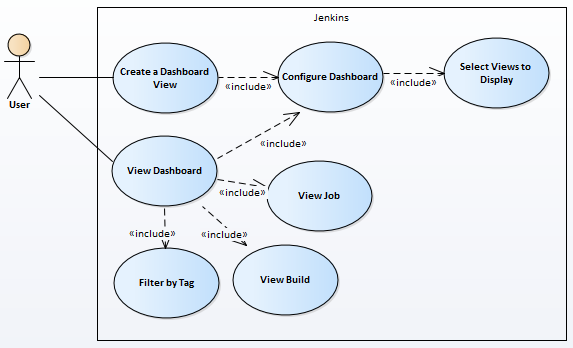
\includegraphics[scale=.5]{figures/usecases.png}}
\caption{Dashboard plugin Use Case diagram}  
\label{fig:usecases}
\end{figure}

The plugin is designed to be as simple as creating a new View inside the tool, selecting which other Views are requested to display. Afterwards, the user can freely change its configuration, namely add, remove or change which views will be displayed.

\subsection{Jenkins Plugin - Filtered Dashboard View}\label{sc:dashboard}

\subsubsection{Mission Control Plugin}\label{mission_plugin}

Accounting that we want to create a Dashboard, we came across the Mission Control Plugin~\cite{jkns:missionC}, that has practically all the base to work with, a full dashboard view that features:

\begin{itemize}
\item Job status display;
\item Build history and build queue;
\item Extends a View Object, which can be added to the main dashboard.
\end{itemize}

Despite being a starting point it needed to be trimmed and adapted to our requirements. 

\subsubsection{Metadata Plugin}\label{metadata_plugin}

Considering that one of the requirements is filtering the data displayed with the information of each test configuration and since Jenkins has the possibility to store information on each of its CI items in XML format, then it could be stored some type of metadata as well.

To facilitate this, we used the extension point that Metadata Plugin~\cite{jkns:metadata} provides, in conjunction with the Jenkins API, to apply relevant filters on each job for an easier parsing of these configurations information.

This Metadata can be applied to Jobs simply through the customization menu, which will apply it to every future Build after this point. 

Or alternatively, automate the process simply by calling a post-build CLI command that is provided from the same plugin.

\subsection{Server Side Implementation Design}\label{sc:implementationDesign}

Understanding how the back end in Java interacts with Jenkins and how projects were organized in Views, we defined a \textit{Top-down} strategy to obtain and parse the information of our items of interest.
This means we had to process View by View as individual projects to relate their child items in our Dashboard as seen in the figure~\ref{fig:dashboardDiagram}.

\begin{figure}[H]
\centerline{\includegraphics[scale=0.28]{figures/dashboardDiagram}}
\caption{\textit{Top-down} approach diagram}  
\label{fig:dashboardDiagram}
\end{figure}

Finally, the addition of Tags to filter the information is the key feature of our Dashboard. This concept helps to maintain track of each configuration, with the minimum requisite of adding, or modifying, these labels to Jobs in the building process.

This design permits a totally scalable structure, since it has no limitations on the number of Views associated to the Dashboard, nor its Jobs and Builds. It can also be extendable to put more information in each of its custom classes for additional metrics and indicators in the future if desired. All this information only depends on the Jenkins API and what it supports.

\subsection{Front-End Implementation Design}\label{sc:frontend}

For information organization structure, in the front-end display of the Dashboard, we based on the same scripts of the Mission Control Plugin, described in section~\ref{mission_plugin}, along with several common Web Application libraries and frameworks such as Javascript, jQuery and Bootstrap, all processed in Apache Jelly, a Java and XML based scripting and processing engine that allows Jenkins its UI to be extended by plugins.

Since the data exported to the API is already well structured, the presentation process was completed with ease, only requiring a way to exhibit the view of a project with an intuitive display. 

To accomplish the aforementioned, was decided to display every Job inside the project as a column in a table, being each row cell its Builds organized in a descending chronological order. Each cell has its Tags associated for a quick reference of the configurations utilized in the respective Build.

\section{Conclusions}\label{sec:conclui}

In the end of this project we were able to develop successfully the intended Dashboard Plugin~\cite{jksn:myplugin}. 

Although narrowed down some features expected in the beginning of the project, such as displaying metrics about the hardware validation process due to time constraints between the end of development and testing  of the Plugin, we believe it will greatly help development teams to keep track of their projects in a simpler and streamlined way. 

%%English version: comment first, uncomment second
%\bibliographystyle{unsrt-pt}  % numeric, unsorted refs
\bibliographystyle{unsrt}  % numeric, unsorted refs
\bibliography{refs}

\end{multicols}

\end{document}
